\documentclass[11pt,letterpaper]{article}
\usepackage{fullpage}

\usepackage[english]{babel}
\usepackage[utf8]{inputenc}
\usepackage{amsmath}
\usepackage{graphicx}
\usepackage[hidelinks]{hyperref}
\usepackage{float}
\usepackage{amsfonts}
\usepackage{algorithm,algpseudocode}
             
\graphicspath{{../results}}
             
\begin{document} 

\title{Experiment 1}
\maketitle

\section*{Simulation Details}

Considered $K = 3$, $T = 5005$, $N = 125$. Report statistics at $t = 1000, 3000, 5000$ \\
\textbf{The Bandit priors that were considered}:
\begin{itemize}
\item Uniform: Draw the mean rewards for the arms from [0.25, 0.75]
\item ``HeavyTail": We took the mean rewards to be randomly drawn from Beta($\alpha=0.6,\beta=0.6$). With this distribution it was likely to have arms that were at the extremes (close to 1 and close to 0) but also some of the arms with intermediate value means.
\item Needle-in-haystack
\begin{enumerate}
\item Medium - 9 arms with mean 0.50, 1 arm with mean 0.55 (+ 0.05)
\item High - 9 arms with mean 0.50, 1 arm with mean 0.70 (+ 0.20)
\end{enumerate}
\end{itemize}
\textbf{Algorithms considered}:
\begin{enumerate}
\item ThompsonSampling with priors of $Beta(1, 1)$ for every arm.
\item DynamicGreedy with priors of $Beta(1, 1)$ for every arm
\item Bayesian Dynamic $\epsilon$-greedy with priors of $Beta(1, 1)$ for every arm and $\epsilon=0.05$
\end{enumerate}
\textbf{Agent Algorithms considered}:
\begin{enumerate}
\item HardMax
\item HardMaxWithRandom
\item SoftMax
\end{enumerate}
\textbf{Memory Sizes}
\begin{enumerate}
\item 10
\item 25
\item 100
\end{enumerate}
\pagebreak
\textbf{Simulation Procedure}
\begin{algorithm}
\begin{algorithmic}[1]
\For{Each prior $p$}
	\For{Each agent algorithm $agent alg$}
		\For{Each principal algorithm pair $principalalg1$, $principalalg2$}
			\For{$N$ simulations}
				\State Generate true distribution from $p$ (except for needle-in-haystack, just use $p$ itself)
				\State Give the agents 5 observations from each principal
				\State Run simulation for T periods
			\EndFor
		\EndFor
	\EndFor
\EndFor
\end{algorithmic}
\end{algorithm}

\pagebreak
\section*{Results}

One thing which is ambiguous to define is the regret value to use when a principal never gets chosen in a given simulation. When calculating any of the aggregate regret statistics we drop these simulations, but we do record how many rounds have an undefined regret. \\
\vspace{0.5cm}

First, we'll restrict focus to $t = 5000$ and look at the performance of ThompsonSampling. Note that the y axis here represents the market share that the ThompsonSampling principal gets. \\
\vspace{0.5cm}

Performance of ThompsonSampling vs DynamicGreedy and DynamicEpsilonGreedy across all agent models, memory sizes, and priors: \\
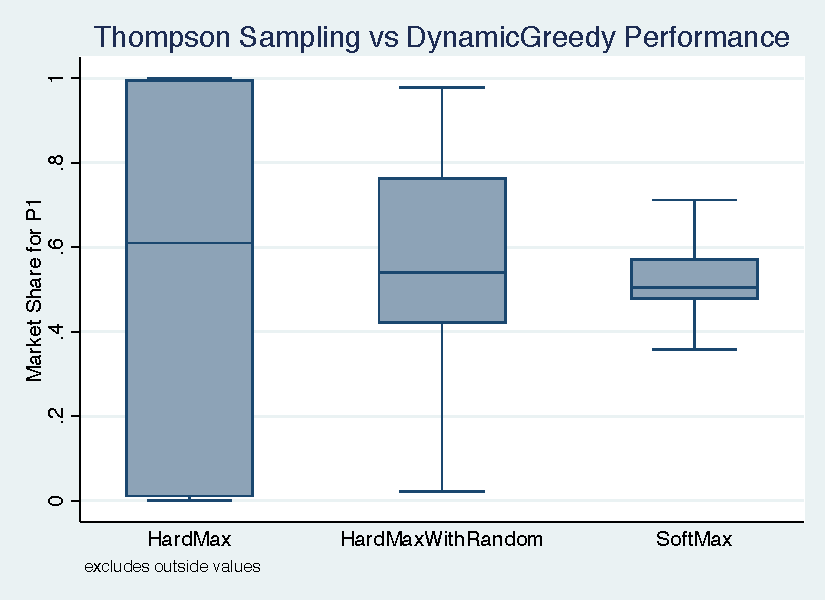
\includegraphics[scale=0.75]{ts_perf_dg} \\
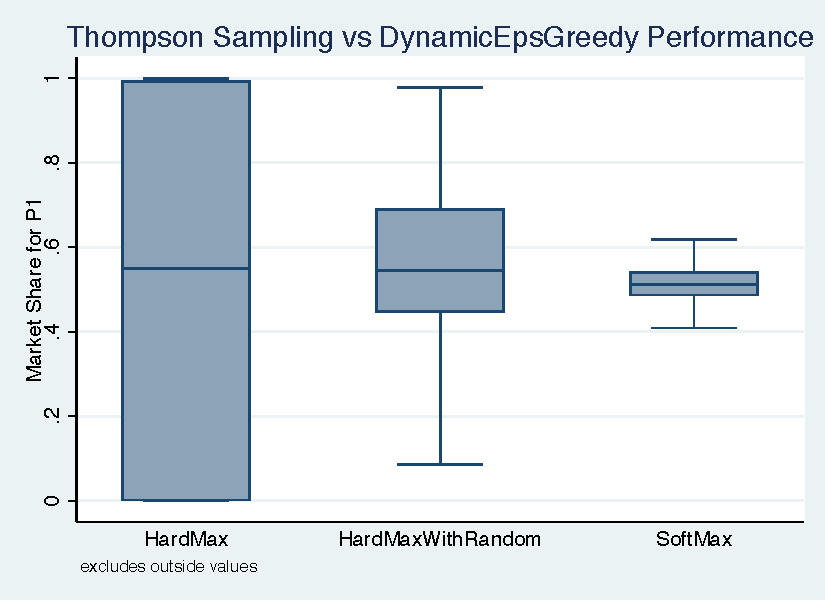
\includegraphics[scale=0.75]{ts_perf_deg} \\

Now, looking across different memory sizes for each agent model (still using each prior): \\
\textbf{HardMax} \\
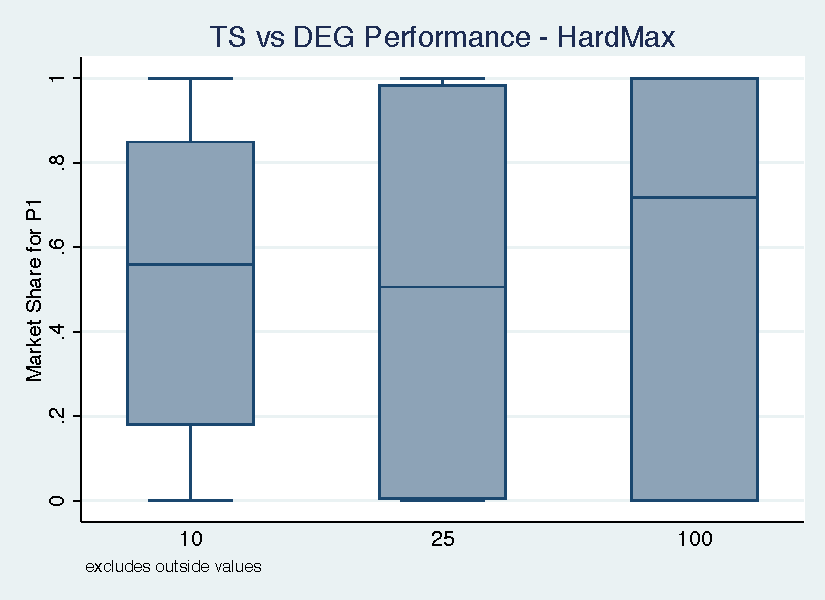
\includegraphics[scale=0.9]{hm_ts_deg} \\
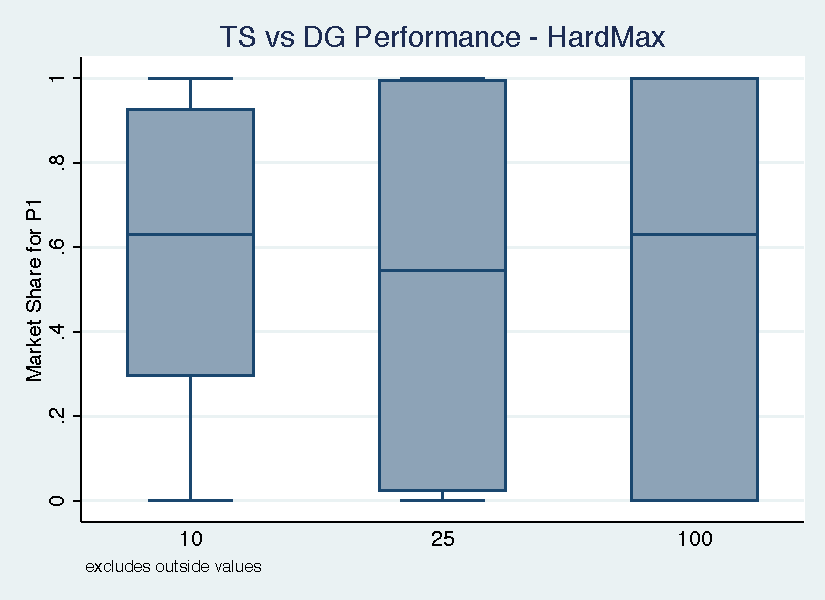
\includegraphics[scale=0.9]{hm_ts_dg} \\
Under HardMax it's clear that there is high variability in market share that is increasing in memory size and indicative of less competition but the median across memory sizes still has ThompsonSampling winning.

\pagebreak
\textbf{HardMaxWithRandom} \\
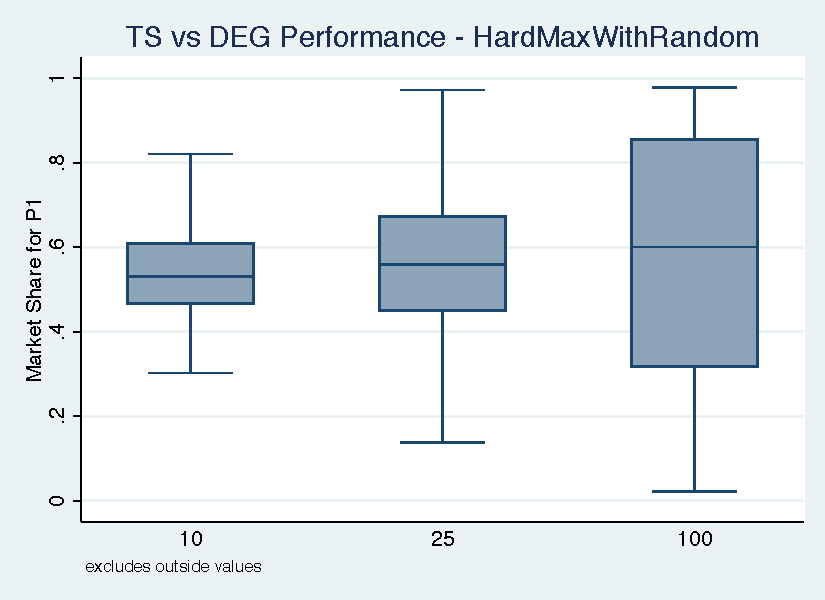
\includegraphics[scale=0.9]{hmr_ts_deg} \\
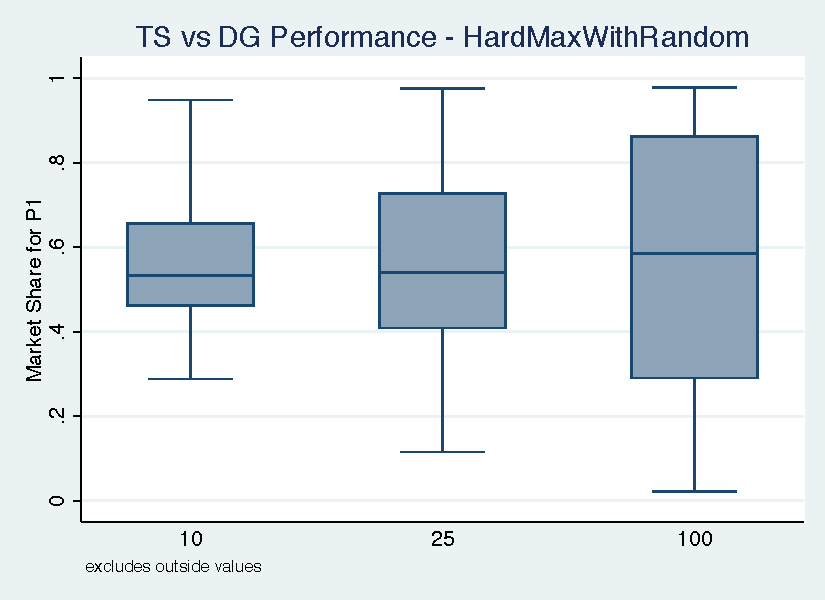
\includegraphics[scale=0.9]{hmr_ts_dg} \\
Under HardMaxWithRandom, the amount of variability decreases (more competition) but is still increasing in memory size and ThompsonSampling still wins in most simulations.

\pagebreak
\textbf{SoftMax} \\
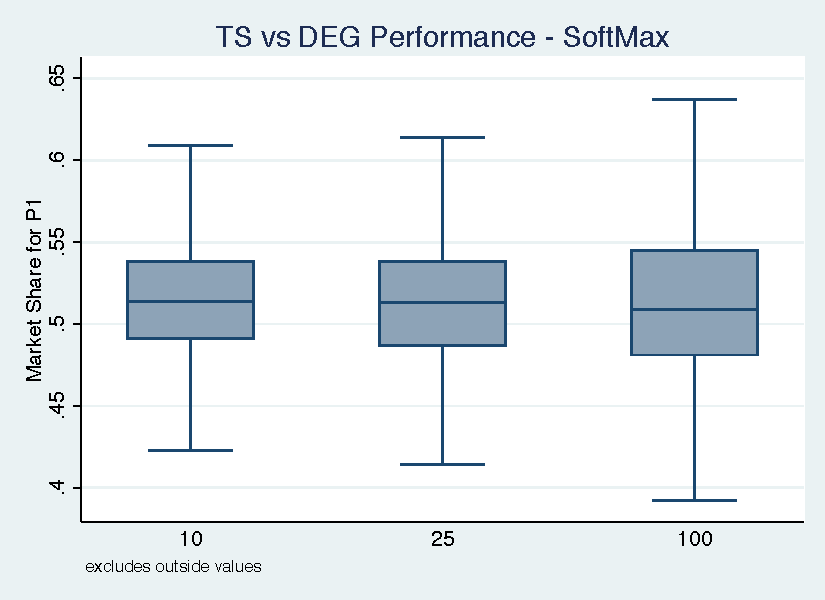
\includegraphics[scale=0.9]{sm_ts_deg} \\
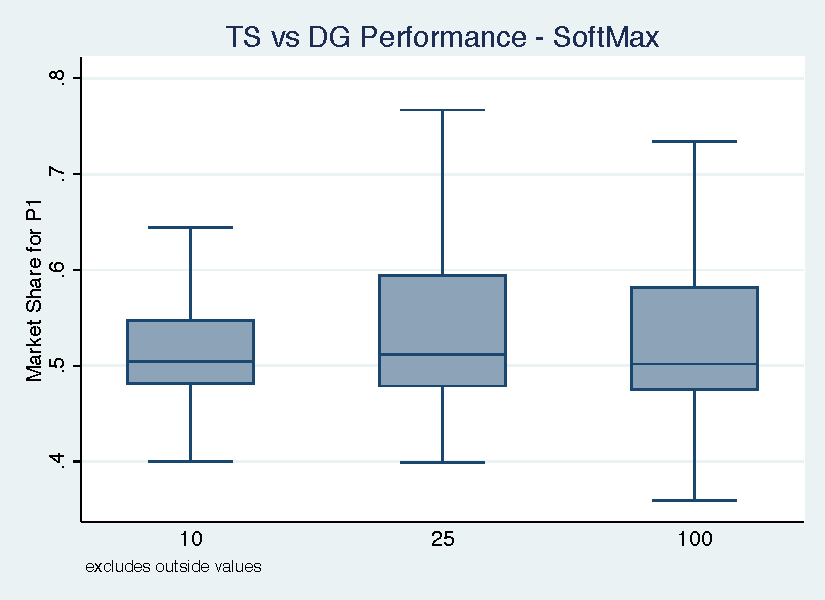
\includegraphics[scale=0.9]{sm_ts_dg} \\
Under SoftMax there is less variability (more competition) that does not change much with memory size and here ThompsonSampling wins more in the median simulation but only a bit.

\pagebreak
We'll now look fix memory size to be 100 and look at the performance across priors.\\
\textbf{HardMax} \\
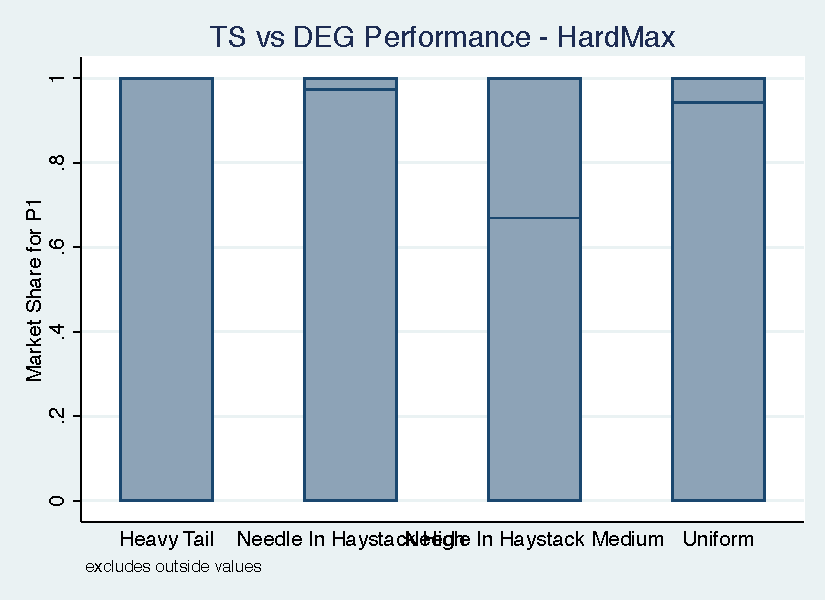
\includegraphics[scale=0.9]{hm_ts_deg_prior} \\
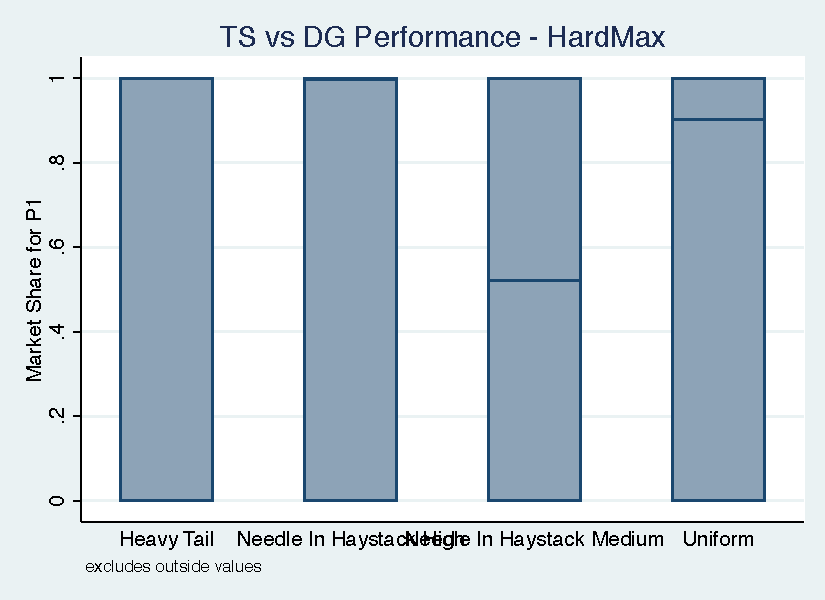
\includegraphics[scale=0.9]{hm_ts_dg_prior} \\
With HardMax there is significant variability (as noted before), but we have that in the needle in haystack medium case the median is approximately 0.5 while in Uniform + Needle in Haystack High the median is 1 and heavy tail it is almost 0. I don't know if this is something interesting or just noise due to the variability in HardMax. Will have to look into this more.

\pagebreak
\textbf{HardMaxWithRandom} \\
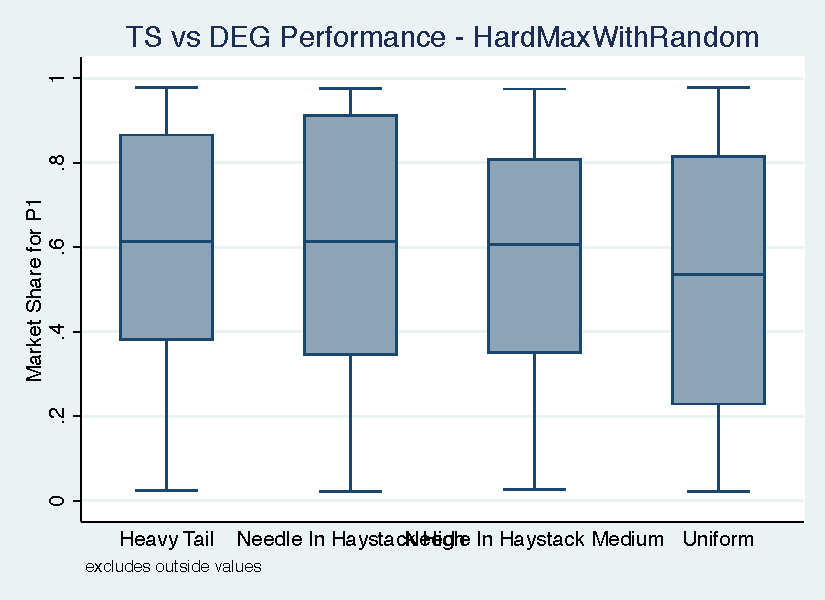
\includegraphics[scale=0.9]{hmr_ts_deg_prior} \\
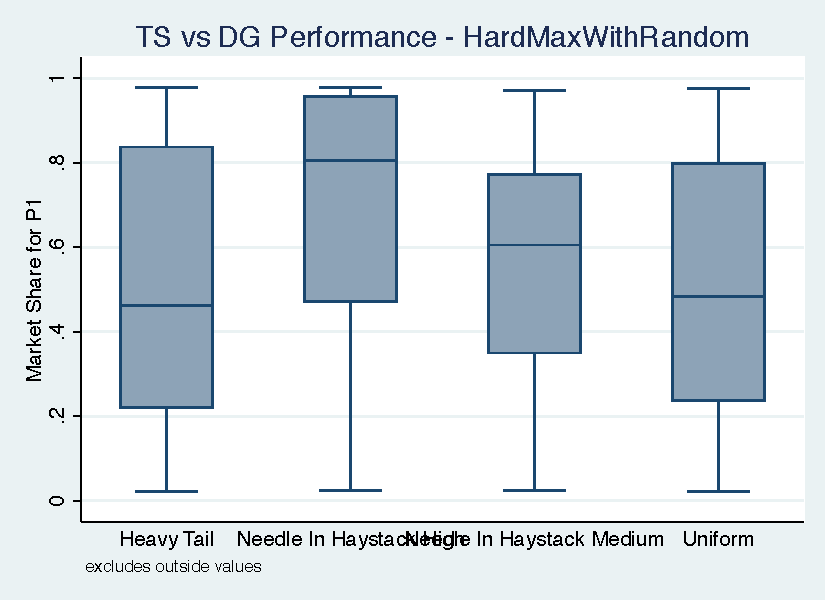
\includegraphics[scale=0.9]{hmr_ts_dg_prior} \\
With TS vs DEG we see roughly the same performance across priors, but for TS vs DG we see as with HardMax that in the needle in haystack high instance we have that TS wins by a lot but not so much in the heavy tail case. This makes sense as TS (and DEG) should generally find the ``good" arm while DG may sometimes wrongly identify the best arm, leading to this disparity.


\pagebreak
\textbf{SoftMax} \\
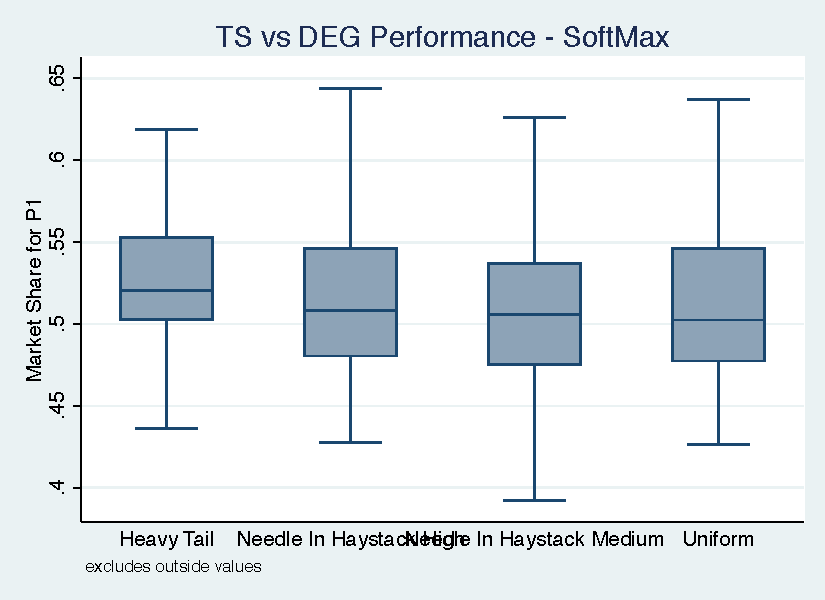
\includegraphics[scale=0.9]{sm_ts_deg_prior} \\
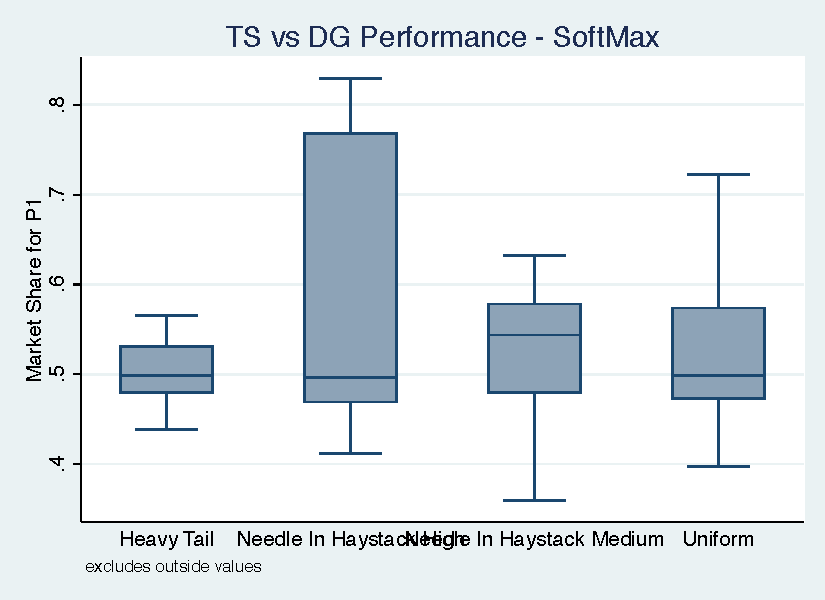
\includegraphics[scale=0.9]{sm_ts_dg_prior} \\
Nothing horribly interesting here besides noting that the same TS vs DG difference appears in the Needle in haystack high prior.


\pagebreak
Now, a couple of plots giving a sense of regret values for ThompsonSampling across different agent algorithms and memory values.\\
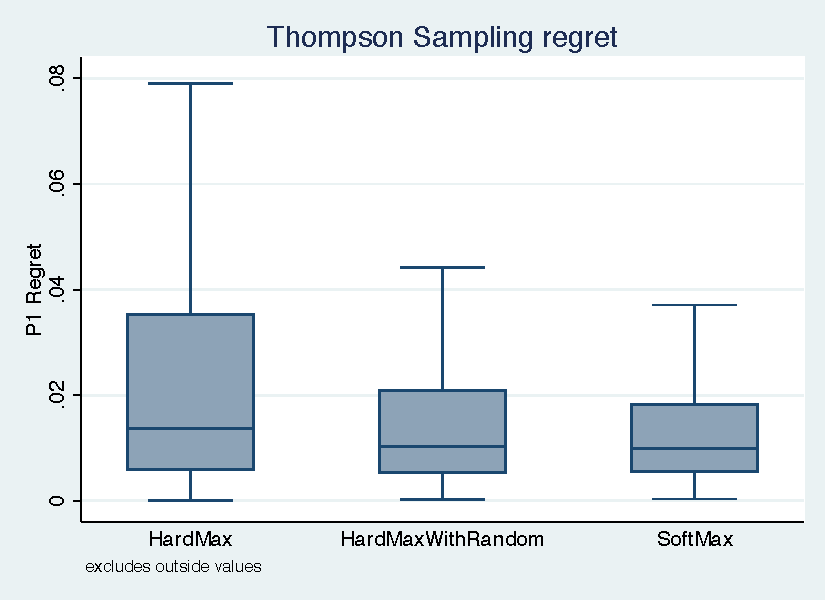
\includegraphics[scale=1]{ts_regret_agent_algs} \\
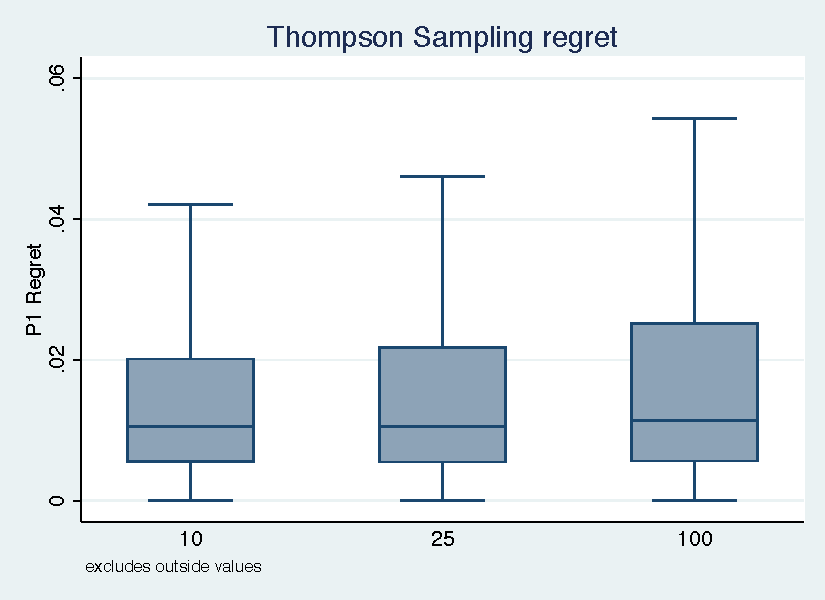
\includegraphics[scale=1]{ts_regret_memory}




\end{document}